\documentclass{beamer}

%\usetheme[headernav]{TACC} %%Drop the 'headernav' if you don't like
                           %%the stuff at the top of your slide
\usetheme[headernav]{TACC}
%\usetheme{default}
%\usetheme{TACC}

\usepackage{amsmath,amssymb,amsthm}
%\usepackage{graphicx} %% Uncomment if you're going to have figures

\title{Source Control Management and Build Systems}
\subtitle{Git and Make}

\event{TACC Summer Supercomputing Institute}

\author{Andy R. Terrel}
\institute{The Texas Advanced Computing Center}

\date{August 2, 2012}  %% Use this if you want to fix the date in
                       %% stone rather than use \today

\begin{document}

\begin{frame}
  \titlepage
\end{frame}

\section*{Outline}% Make it easy to jump to this page in the PDF

% use outline_currentsection.tex to highlight the current section

% Auto-generate the TOC slide(s)
\begin{frame}
  %\tableofcontents[currentsection]
  \tableofcontents
\end{frame}



\section{Git}
\subsection{Source Control Management}
% Auto-generate the TOC slide(s)
\begin{frame}
  \tableofcontents[currentsection, currentsubsection]
  %\tableofcontents
\end{frame}


\setbeamercolor{normal text}{fg=gray,bg=}
\setbeamercolor{alerted text}{fg=black,bg=}

\begin{frame}
Why use source control managment?
\usebeamercolor{normal text}
  \begin{itemize}
    \item \alert<+>{Traceability, know when things were added.}
    \item \alert<+>{Reproducibility, know what code was run when.}
    \item \alert<+>{Collaboration, allow contributions without risking code breakage.}
  \end{itemize}
\end{frame}

\subsubsection{Local Source Control Management}
\begin{frame}
\begin{columns}[c]
\column{2in}
\framebox{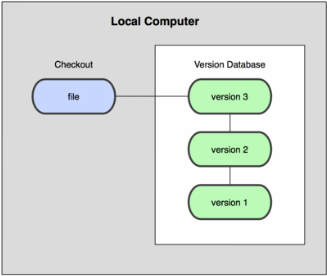
\includegraphics[scale=.5]{../figures/git/local_scm.png}}
\column{2in}
\only<1-3>{
\usebeamercolor{normal text}
\begin{itemize}
\item \alert<+>{Edit and revise local files.}
\item \alert<+>{Keep versions of the file that can be ``checked out''.}
\item \alert<+>{Use smart tools to see differences in the files.}
\end{itemize}
}
\only<4>{
Examples:
\begin{itemize}
\item{SCCS (1972)}
\item{RCS (1982)}
\end{itemize}
}
\end{columns}
\end{frame}

\subsubsection{Centralized Source Control Management}
\begin{frame}
\begin{columns}[c]
\column{2in}
\only<1-3>{
\usebeamercolor{normal text}
\begin{itemize}
\item \alert<+>{Same interactions as local SCM.}
\item \alert<+>{Diffs stored on central resource for access management.}
\item \alert<+>{Easy to work on same code at the same time.}
\end{itemize}
}
\only<4>{
Examples:
\begin{itemize}
\item{CVS (1989)}
\item{SVN (2000)}
\item{ClearCase}
\item{Perforce}
\end{itemize}
}
\column{2.5in}
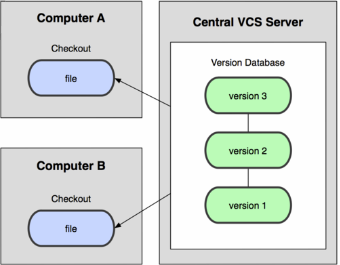
\includegraphics[scale=.5]{../figures/git/centralized_scm.png}
\end{columns}
\end{frame}

\subsubsection{Distributed Source Control Management}
\begin{frame}
\begin{columns}
\column{2in}
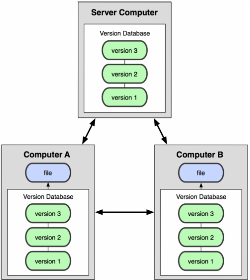
\includegraphics[scale=.5]{../figures/git/distributed_scm.png}
\column{2in}
\only<1-3>{
\usebeamercolor{normal text}
\begin{itemize}
\item \alert<+>{Edit and revise local files, but also keep version database local}
\item \alert<+>{Easy to give full repository to collaborators.}
\item \alert<+>{Completely distributed allowing for a several workflow styles.}
\end{itemize}
}
\only<4>{
Examples:
\begin{itemize}
\item{Bitkeeper (2000)}
\item{Darcs (2003)}
\item{Git (2005)}
\item{Bazaar (2005)}
\item{Mercurial (2005)}
\end{itemize}
}
\end{columns}
\end{frame}

\begin{frame}
\begin{center}
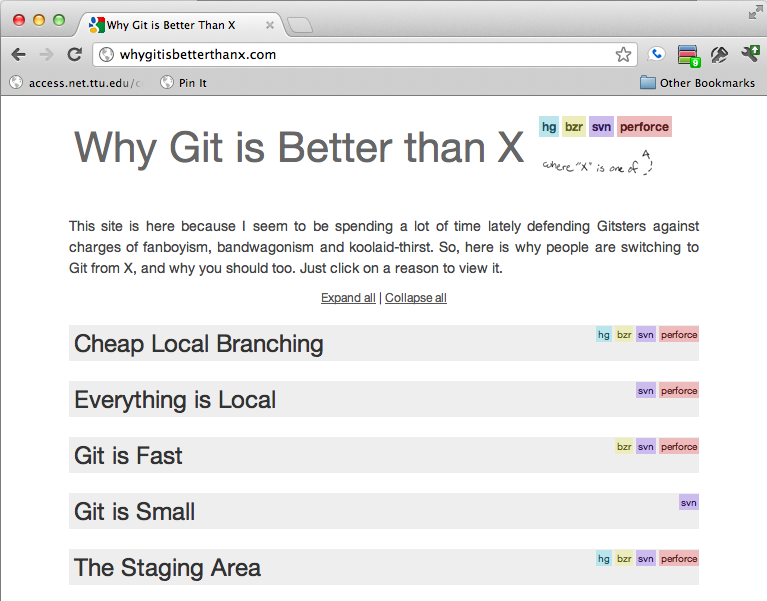
\includegraphics[scale=.4]{../figures/git/whygitisbetter.png}
\end{center}
\end{frame}

\subsection{Local Command Demo}
% Auto-generate the TOC slide(s)
\begin{frame}
  \tableofcontents[currentsection, currentsubsection]
  %\tableofcontents
\end{frame}

\begin{frame}[fragile]
\begin{verbatim}
$ ssh lonestar.tacc.utexas.edu
$ module load git
$ git help
usage: git ...
$ git help init
GIT-INIT(1)                        Git Manual                       GIT-INIT(1)
...q
$ git config --global user.name "John Doe"
$ git config --global user.email johndoe@example.com
\end{verbatim}
\end{frame}
\begin{frame}[fragile]
\begin{block}{git init}
Create an empty git repository or reinitialize an existing one
\end{block}
\begin{verbatim}
$ mkdir git_test
$ cd git_test
$ git init
Initialized empty Git repository in
/home1/01392/aterrel/git_test/.git/
\end{verbatim}
\end{frame}

\begin{frame}[fragile]
\begin{block}{git add}
Add file contents to the index
\end{block}
\begin{verbatim}
$ echo "Hello Git World" >> README
$ git add README
\end{verbatim}
\end{frame}

\begin{frame}[fragile]
\begin{block}{git status}
Show the working tree status
\end{block}
\begin{verbatim}
$ git status
# On branch master
#
# Initial commit
#
# Changes to be committed:
#   (use "git rm --cached <file>..." to unstage)
#
#	new file:   README
#
\end{verbatim}
\end{frame}

\begin{frame}[fragile]
\begin{block}{git commit}
Record changes to the repository
\end{block}
\begin{verbatim}
$ git commit -m "Adding README"
[master (root-commit) 774c810] Adding README
 1 file changed, 1 insertion(+)
 create mode 100644 README
\end{verbatim}
\end{frame}

\begin{frame}[fragile]
\begin{block}{git log}
Show the commit logs
\end{block}
\begin{verbatim}
$ git log
commit 774c81087d052e43a630db7f676cfd9a6b006772
Author: Andy R. Terrel <andy.terrel@gmail.com>
Date:   Tue Jul 24 17:53:04 2012 -0500

    Adding README
\end{verbatim}
\end{frame}

\begin{frame}[fragile]
\begin{verbatim}
$ echo "Line 2" >> README
$ git add README
$ git commit -m "Adding Line 2"
$ echo "Line 3" >> README
$ git add README
$ git commit -m "Adding Line 3"
$ echo "Clear file" > README
$ git add README
$ git commit -m "Clear file"
\end{verbatim}
\end{frame}

\begin{frame}[fragile]
\tiny
\begin{verbatim}
$ git log
commit c0513dbf6b609715f1510c438b9d00f065f7f3f4
Author: Andy R. Terrel <andy.terrel@gmail.com>
Date:   Tue Jul 24 17:58:53 2012 -0500

    Clear file

commit 88d4a87be3e7444d06463108e98ca78802f4859e
Author: Andy R. Terrel <andy.terrel@gmail.com>
Date:   Tue Jul 24 17:58:25 2012 -0500

    Adding Line 3

commit 43a446bedd92946d0ccf6fa2218f623284695f8b
Author: Andy R. Terrel <andy.terrel@gmail.com>
Date:   Tue Jul 24 17:58:01 2012 -0500

    Adding Line 2

commit 774c81087d052e43a630db7f676cfd9a6b006772
Author: Andy R. Terrel <andy.terrel@gmail.com>
Date:   Tue Jul 24 17:53:04 2012 -0500

    Adding README
\end{verbatim}
\end{frame}

\begin{frame}[fragile]
\begin{block}{git diff}
Show changes between commits, commit and working tree, etc
\end{block}
\begin{verbatim}
$ git diff 88d4a87be3
diff --git a/README b/README
index d5c15a2..fcb6062 100644
--- a/README
+++ b/README
@@ -1,3 +1 @@
-Hello Git World
-Line 2
-Line 3
+Clear file
\end{verbatim}
\end{frame}

\begin{frame}[fragile]
\begin{block}{git reset}
Reset current HEAD to the specified state
\end{block}
\begin{verbatim}
$ git reset 43a446bedd92
README: needs update

< fix file >
$ git add README
$ git commit -m "Don't clear line this time"
Created commit 0c1757b: Don't clear line this time
 1 files changed, 2 insertions(+), 2 deletions(-)
\end{verbatim}
\end{frame}

\begin{frame}[fragile]
\begin{block}{git checkout}
Checkout a branch or paths to the working tree
\end{block}
\begin{verbatim}
$ git checkout 43a446bedd9294 -- README

$ cat README
Hello Git World
Line 2
$ git add README
$ git commit -m "Going back to line 2"
Created commit e56f835: Going back to line 2
 1 files changed, 2 insertions(+), 2 deletions(-)
\end{verbatim}
\end{frame}

\begin{frame}[fragile]
\begin{block}{git checkout}
Checkout a branch or paths to the working tree
\end{block}
\tiny
\begin{verbatim}
$ git checkout 88d4a87be3e7
Note: checking out '88d4a87be3e7'.

You are in 'detached HEAD' state. You can look around, make experimental
changes and commit them, and you can discard any commits you make in this
state without impacting any branches by performing another checkout.

If you want to create a new branch to retain commits you create, you may
do so (now or later) by using -b with the checkout command again. Example:

  git checkout -b new_branch_name

HEAD is now at 88d4a87... Adding Line 3

$ git checkout master
Previous HEAD position was 88d4a87... Adding Line 3
Switched to branch 'master'
\end{verbatim}
\end{frame}

\subsection{Remote Command Demo}
% Auto-generate the TOC slide(s)
\begin{frame}
  \tableofcontents[currentsection, currentsubsection]
  %\tableofcontents
\end{frame}

\begin{frame}[fragile]
\begin{block}{git clone}
Clone a repository into a new directory
\end{block}
\begin{block}{git pull}
Fetch from and merge with another repository or a local branch
\end{block}
\begin{block}{git push}
Update remote refs along with associated objects
\end{block}
\end{frame}


\subsection{Resources}
% Auto-generate the TOC slide(s)
\begin{frame}
  \tableofcontents[currentsection, currentsubsection]
  %\tableofcontents
\end{frame}

\begin{frame}[fragile]
\tiny
\begin{verbatim}
$ git help -a
usage: git [--version] [--exec-path[=GIT_EXEC_PATH]] [-p|--paginate|--no-pager] [--bare] [--git-dir=GIT_DIR] [--work-tree=GIT_WORK_TREE] [--help] COMMAND [ARGS]

available git commands in '/usr/bin'
------------------------------------
  add                 diff-index          ls-files            patch-id            shortlog
  add--interactive    diff-tree           ls-remote           peek-remote         show
  am                  fast-export         ls-tree             prune               show-branch
  annotate            fast-import         mailinfo            prune-packed        show-index
  apply               fetch               mailsplit           pull                show-ref
  archive             fetch--tool         merge               push                stash
  bisect              fetch-pack          merge-base          quiltimport         status
  blame               filter-branch       merge-file          read-tree           stripspace
  branch              fmt-merge-msg       merge-index         rebase              submodule
  bundle              for-each-ref        merge-octopus       rebase--interactive symbolic-ref
  cat-file            format-patch        merge-one-file      receive-pack        tag
  check-attr          fsck                merge-ours          reflog              tar-tree
  check-ref-format    fsck-objects        merge-recursive     relink              unpack-file
  checkout            gc                  merge-resolve       remote              unpack-objects
  checkout-index      get-tar-commit-id   merge-stupid        repack              update-index
  cherry              grep                merge-subtree       repo-config         update-ref
  cherry-pick         hash-object         merge-tree          request-pull        update-server-info
  clean               http-fetch          mergetool           rerere              upload-archive
  clone               http-push           mktag               reset               upload-pack
  commit              imap-send           mktree              rev-list            var
  commit-tree         index-pack          mv                  rev-parse           verify-pack
  config              init                name-rev            revert              verify-tag
  count-objects       init-db             pack-objects        rm                  web--browse
  describe            instaweb            pack-redundant      send-pack           whatchanged
  diff                log                 pack-refs           sh-setup            write-tree
  diff-files          lost-found          parse-remote        shell

\end{verbatim}
\end{frame}

\begin{frame}
\begin{block}{Online Resources}
  \begin{itemize}
  \item \url{http://git-scm.com/book}: very gentle book and other tutorials
  \item \url{http://github.com} and \url{http://bitbucket.org} git web-hosting
  \end{itemize}
\end{block}

\end{frame}



\section{Make}
\end{document}
